
	
	
\chapter{Etude de l'art }
\newpage
	
\section{Introduction}

	
	
\section{Définition d'un drone}
	
Les drones (du mot anglais signifiant « faux bourdon ») sont des aéronefs sans équipage dont le pilotage est automatique ou télécommandé. Leur masse varie de quelques grammes à plusieurs tonnes[10], moins chers et plus simples à mettre en œuvre qu'un avion. Ils sont plus discrets et leur perte est moins grave que celle d'un appareil de son pilote.  !!!!!
	
	
	
	\section{Les types des drones}
	Il existe plusieurs types de drones, nous avons mis l'accent sur deux types:
	\begin{itemize}
	 \item Aile fixe.
	 \item Multirotors 
	\end{itemize}
	\subsection{Aile fixe }
	L'avion à voile fixe est capable de voler en utilisant des ailes qui génèrent une élévation causée par la vitesse avant du véhicule et la forme des ailes.
	
	
	\begin{figure}[h] 
	\begin{center} 
		\centering
 \fbox{	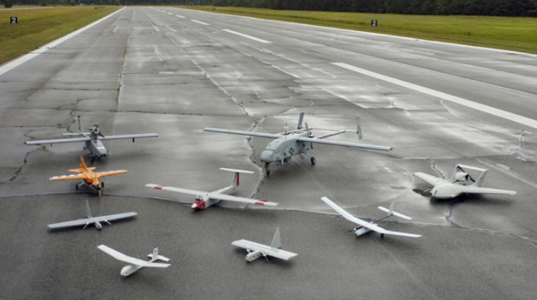
\includegraphics[width=0.6\linewidth]{Images/Ailes fixed}}
		
	\end{center}
	
	\caption{Ailes fixes Drones}
	\end{figure}
	\subsection{Multi-rotors}
	C'est le type de drone qui possède plusieurs rotors sur son corps. Cette caractéristique lui offre la possibilité de rester en position unique pendant une longue période. En plus, ces drones sont très pratiques pour diverses utilisations.
	\begin {figure}[h] 
	\begin{center} 
		\centering
	\fbox{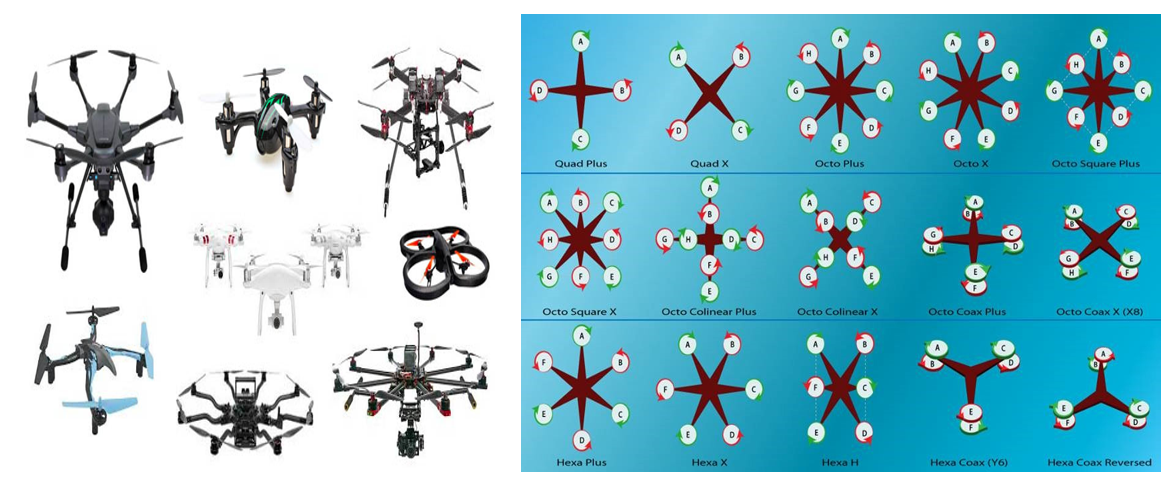
\includegraphics[width=1.1\linewidth]{Images/Types des multirotor}}
		
	\end{center}
	
	\caption{Types des multirotors}
	\end{figure}
	
	
	
	
	
	
	
	\subsection{Comparaison entre aile fixe drone et multirotors drone}
	Après avoir étudié chaque type de drone, nous avons effectué une étude comparative entre eux en terme de vitesse, niveau de contrôle, capacité de charge, endurance et atterissage/décollage.
	
	Nous remarquons à travers ce tableau que les drones à voilure fixe sont plus rapides que les drones à voilure tournante  . Ils sont difficiles à contrôller, supportent une faible charge et nécessitent des grandes surfaces pour l'atterissage et le décollage.
    Vu que notre situation nécessite une vitesse adapté à notre système de détection des oranges, nous avons choisi le quadrirotor qui est facile à contrôler, supporte une charge importante et pratique dans les petites surfaces.      
	\begin{table}[h]
		\begin{center}
			\caption{Comparaison entre fixed wing drone et multirotors drone	 }
			\begin{tabular}{|c|c|c|}
				\hline
				\centering
				& 
				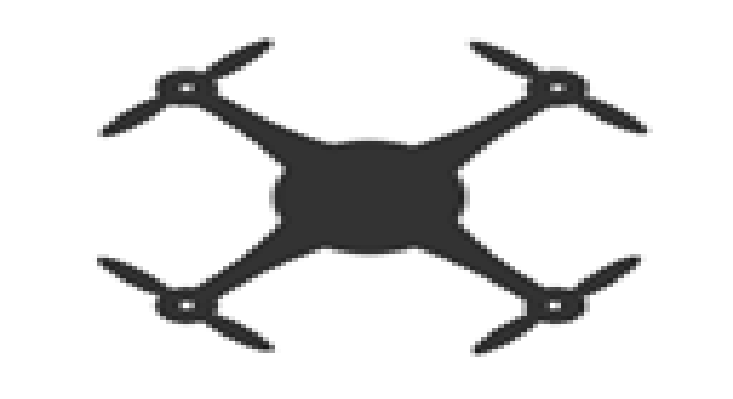
\includegraphics[scale=0.2]{Images/Quadrirotor}
				&
				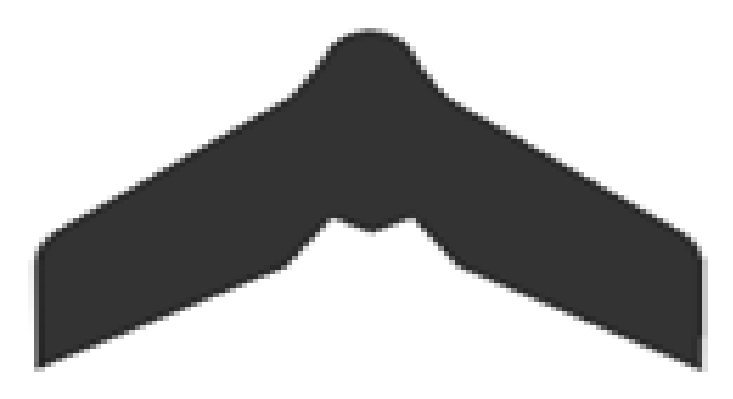
\includegraphics[scale=0.2]{Images/Ailed fixed}\\
				
				\hline
				Vitesse & 70 Km /h - 250 Km /h & 100 Km /h-700 Km /h  \\
				\hline
				Contrôle	& facile &	Difficile \\
				\hline
				Capacité de Charge &	Grande charge &	Petite charge \\
				\hline
				Endurance &	15min-60min & 1h-12heures \\
				\hline
				Atterrissage et décollage &	Petites surfaces &	Grandes surfaces \\
				\hline
			\end{tabular}
		\end{center}
	\end{table}
\newpage
	
	\subsection{Définition du quadrirotor}
Un quadrirotor est un aéronef à voilure tournante à quatre rotors qui sont généralement placés à l'extrémité de la croix. Pour empêcher l'appareil de tourner sur lui-même autour de son axe de lacet, il faut que deux hélices tournent dans un sens et les deux autres dans l'autre. Pour pouvoir diriger l'appareil, il faut placer chaque paire d'hélices qui tournent dans le même sens aux extrémités opposées de la branche transversale.
	\begin{figure}[h] 
	\begin{center} 
		\centering
\fbox{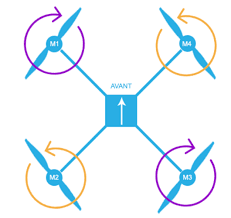
\includegraphics[width=0.6\linewidth]{Images/Sens de rotation des moteurs}}	
	\end{center}
	\caption{Sens de rotation des moteurs }
	\end{figure}
	\section{Histoire des quadrirotors}
	Le premier quadrirotor à décoller du sol est le gyroplane Breguet-Richet, développé par la société Breguet en 1907. Il ne décolle qu'à une hauteur de 60 cm et quatre hommes maintiennent la structure(6). 
	\begin{figure}[h] 
	\begin{center} 
		\centering
	\fbox{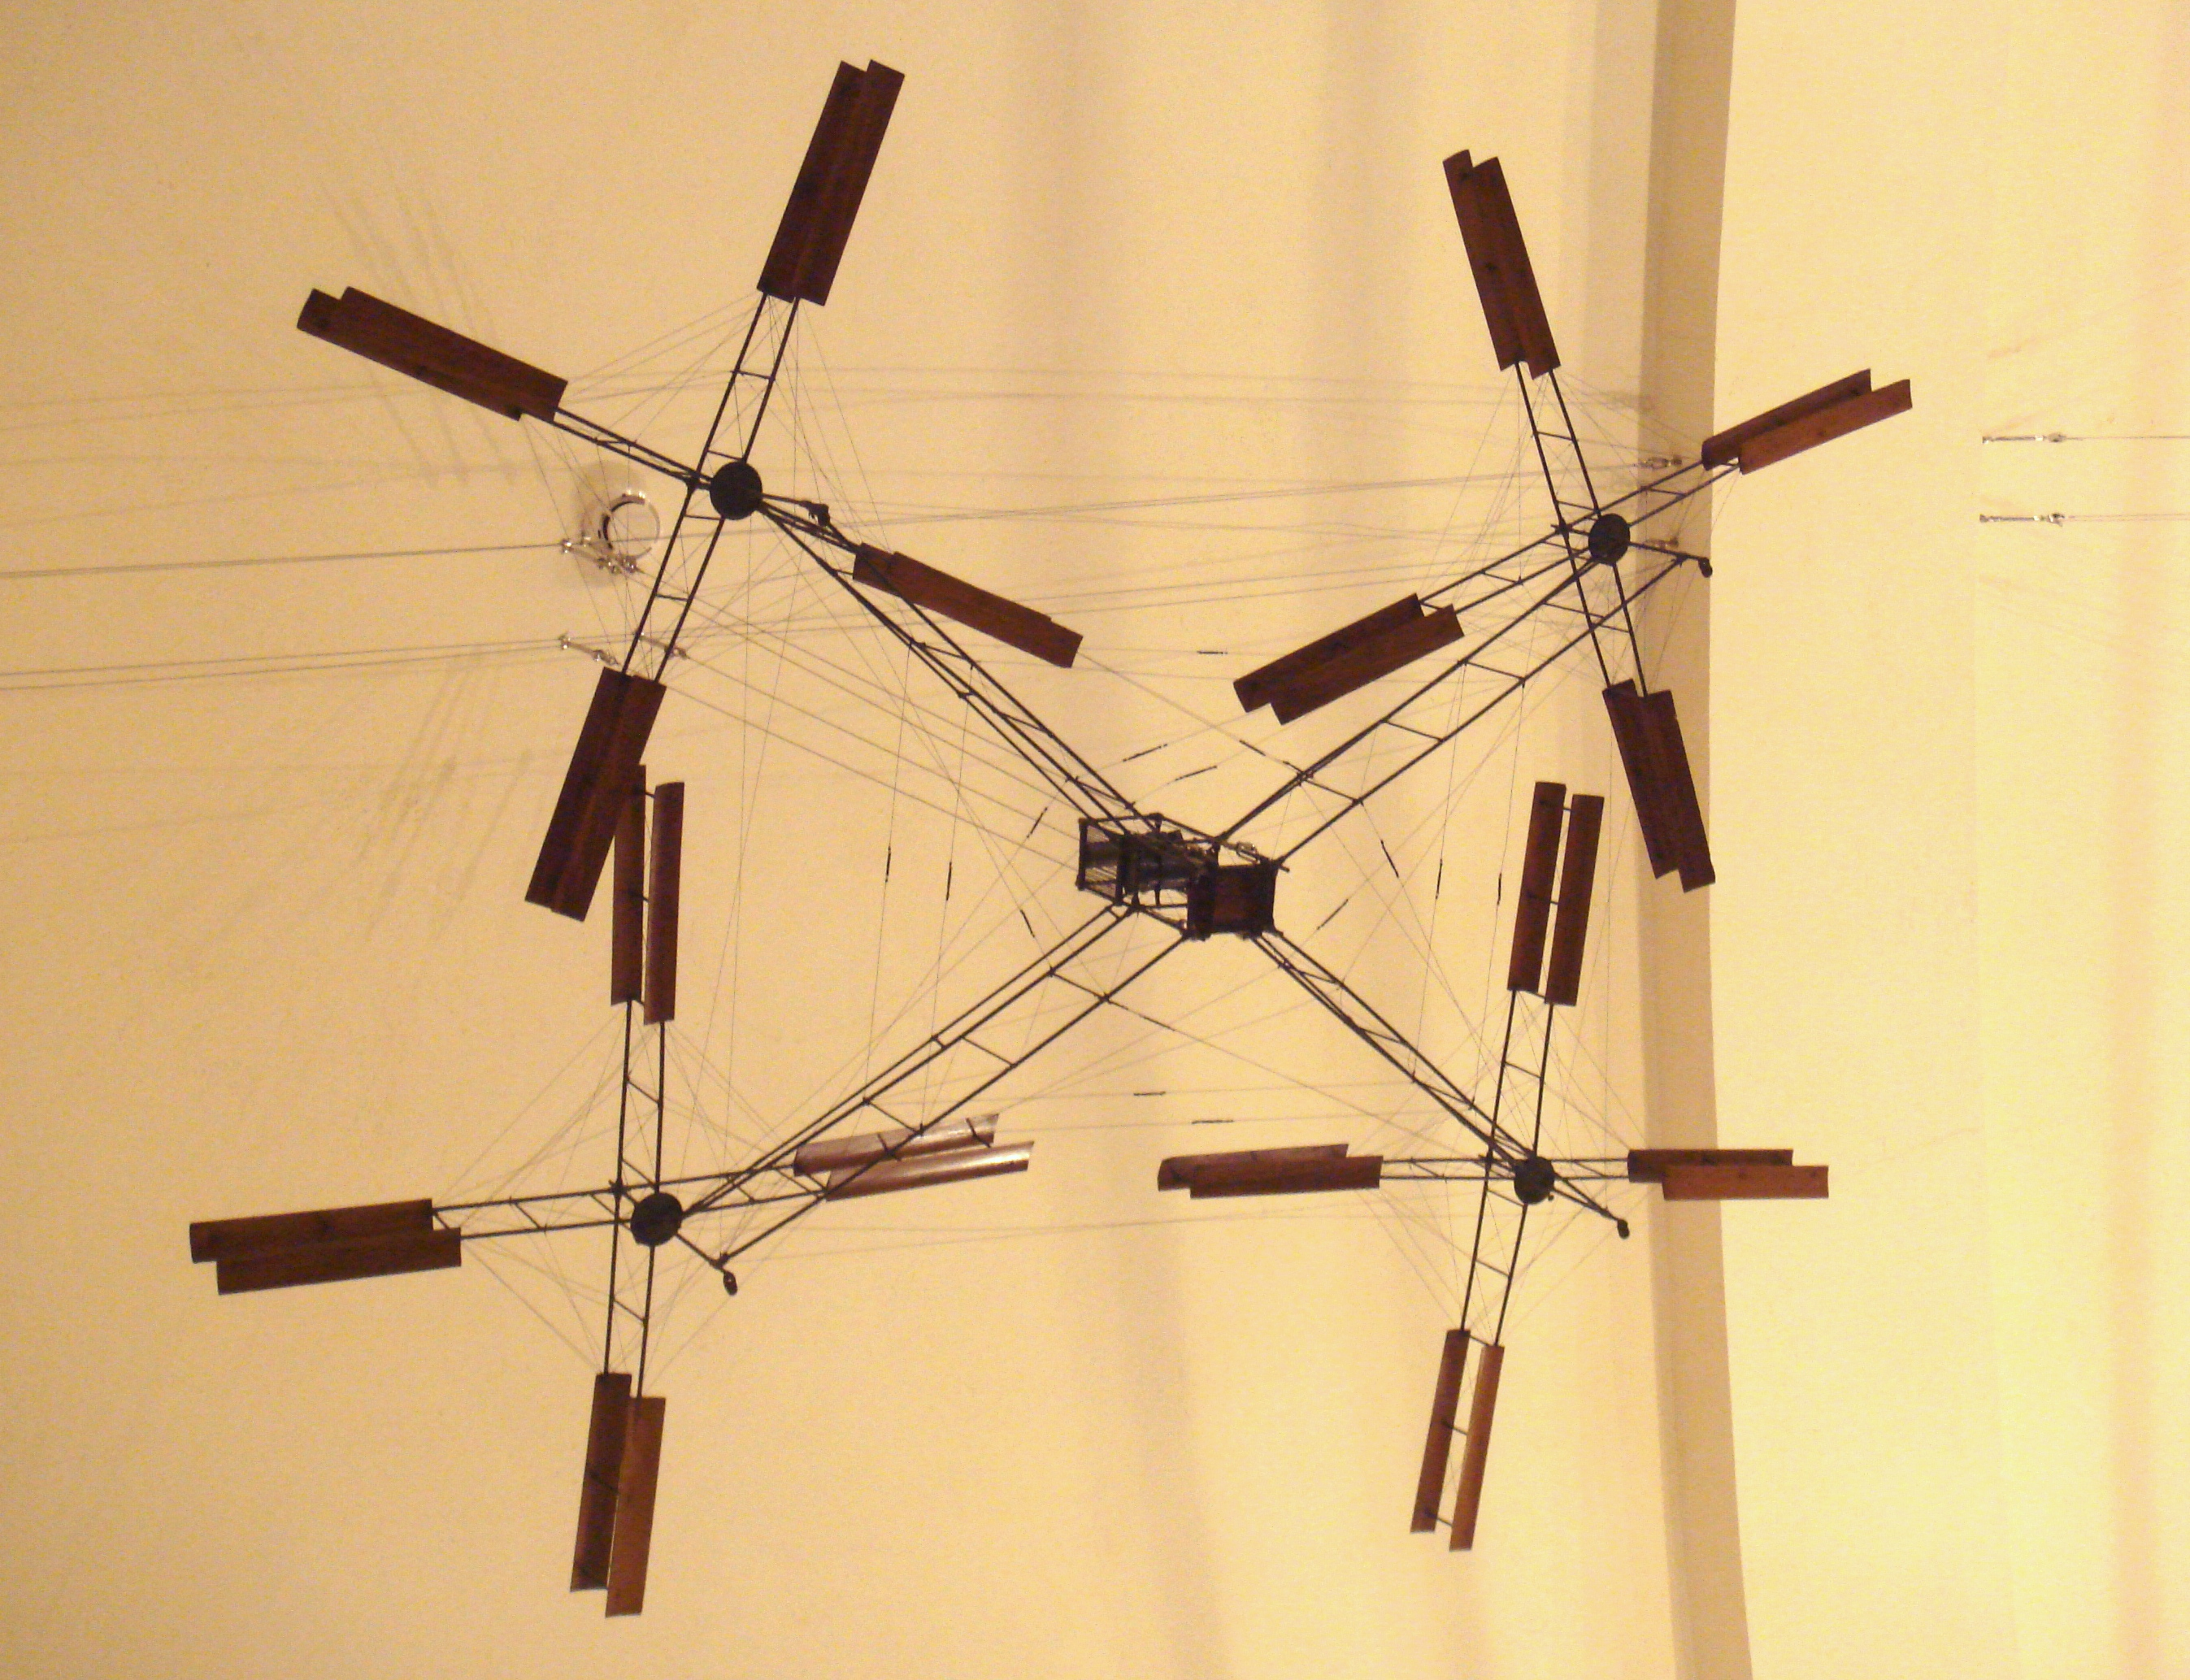
\includegraphics[width=0.6\linewidth]{Images/Breguet_Gyroplane_1907}}
		
	\end{center}
	\caption{Le Gyroplane }
	\end{figure}

	\section{Les domaines d'applications du quadrirotor}
	
	Le quadricoptère est de plus en plus répandu dans le secteur professionnel grâce à son apport de nouvelles informations, son autonomie et sa rapidité. Parmi ses différents domaines d'applications, nous citons: 
	
	\begin{itemize}
		
		\item Le Militaire et la protection civile.
		\item La sécurité et la surveillance.
		\item L'agriculture.
		\item Le Journalisme.
		\item Le FPV racing.
		
	\end{itemize}
	\newpage
	\section{Mouvements du quadrirotor}
	Les mouvements de base du quadrirotor sont réalisés en variant la vitesse de chaque rotor et en changeant la poussée produite. Ces mouvements sont couplés, ce qui signifie que le quadrirotor ne peut pas faire de translation sans réaliser un mouvement de roulis ou de tangage.
	
	Nous présentons ci-dessous les mouvements effectués par le quadrirotor:		
	\begin{itemize}
		\item Mouvement vertical.
		\item Mouvement de roulis.
		\item Mouvement de tangage.
		\item Mouvement de lacet.
	\end{itemize}
	\begin{figure} [h]
	\begin{center}
		\centering
	\fbox{	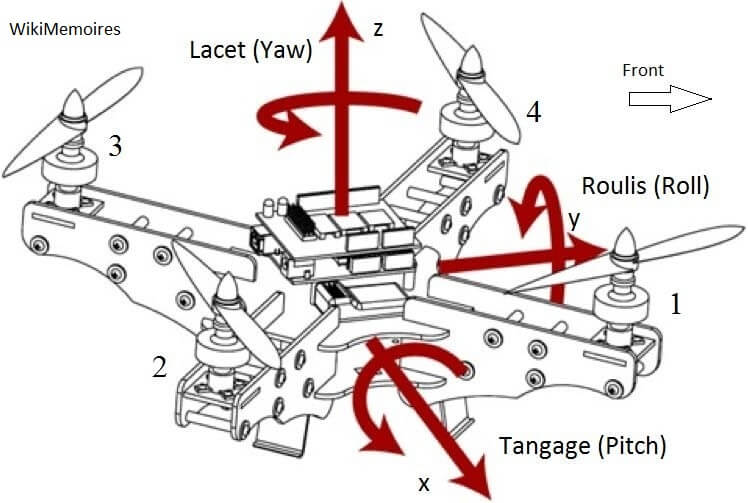
\includegraphics[width=0.7\linewidth]{Images/Les mouvements du drones}}
	\end{center}
	\caption{Les mouvements du drones }
	\end{figure}

	
	\subsection{Mouvement vertical}
	Pour monter, nous augmentons la vitesse des moteurs simultanément, tous les moteurs tournent au même régime et inversement pour descendre. Cette manipulation s'effectue à travers la commande des gaz.
	\begin{figure} [h]
	\begin{center}
		\centering
	\fbox{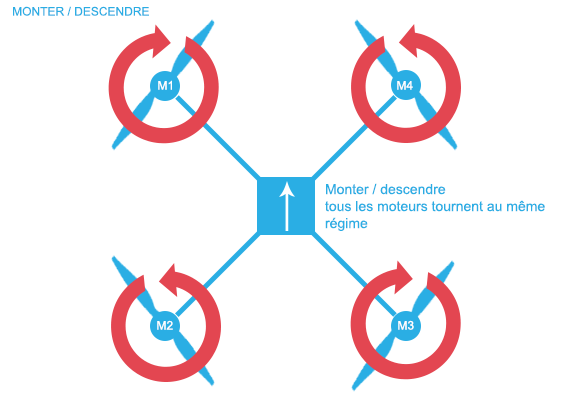
\includegraphics[width=0.6\linewidth]{Images/Mouvement vertical}}
	\end{center}
	\caption{Mouvement vertical}
	\end{figure}
	\newpage
	\subsection{Mouvement de roulis}
	Pour incliner vers la gauche, nous diminuons les moteurs de gauche et augmentons ceux de droite. Inversement pour incliner vers la droite. Cette action s’appelle le roulie.
	\begin{figure} [h]
	\begin{center}
	\fbox{	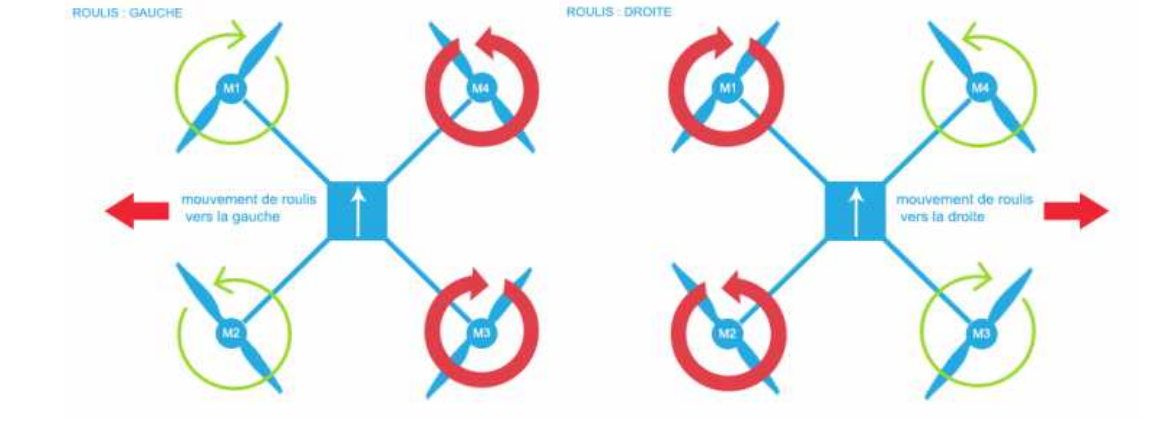
\includegraphics[width=1.1\linewidth]{Images/Mouvement de roulis}}
		\caption{Mouvement de roulis}
	\end{center}
	\end{figure}
	\subsection{Mouvement de tanguage}
	Pour avancer, nous diminuons la vitesse des moteurs avant et augmentons la vitesse des moteurs arrière et inversement pour reculer. Cette action s'appelle le tangage.
	
	
	\begin{figure}[h] 
	\begin{center}
		\centering
		\fbox{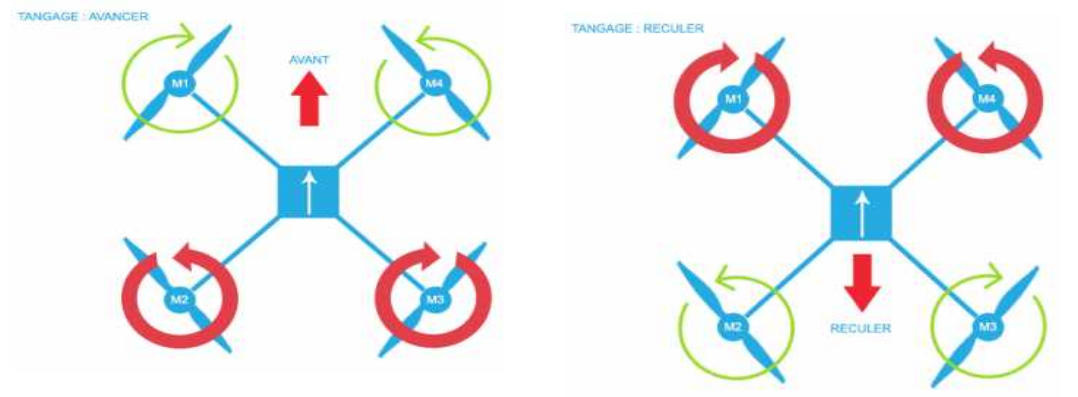
\includegraphics[width=1\linewidth]{Images/Mouvement de tanguage}}
	\end{center}
	\caption{Mouvement de tanguage}
	\end{figure}
	
	\subsection{Mouvement de lacet}
	Pour un mouvement de rotation, nous augmentons la vitesse d’une paire de moteurs sur le même axe et inversement. Ceci est un mouvement de lacet.
	\begin{figure} [h]
	\begin{center}
\fbox{	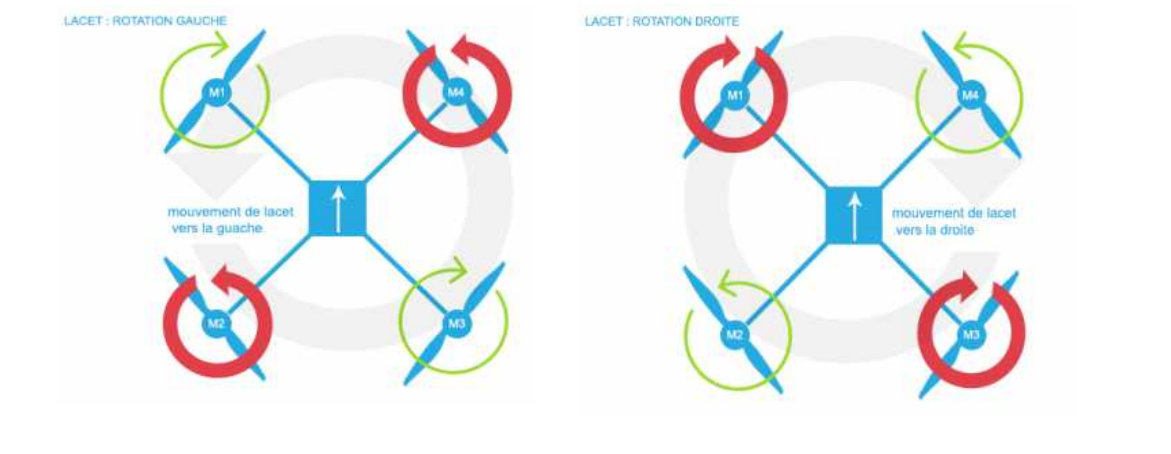
\includegraphics[width=1.1\linewidth]{Images/Mouvement de lacet}}
	\end{center}
	\caption{Mouvement de lacet}	
\end{figure}
\newpage
\subsection {Action PID} !!!!!!!!!!!!
Le régulateur PID combine les trois actions vues précédemment et permet ainsi d’avoir de
bonnes performances aussi bien en vitesse, en stabilité et en précision. L’expression d’un régulateur PID est donné comme suit :

$ c(t)=K_p\times \epsilon(t) + K_i\int\epsilon(t)dt+K_d\frac{d\epsilon(t)}{dt}$


Ainsi ce régulateur permet d’atteindre les objectifs fixés en termes de vitesse de stabilité et de
précision et ce en trouvant la configuration optimale des valeurs des différents gains $K_p $, $ K_i$ et $ K_d$.
\subsection {Action proportionnelle}
L’effet de l’action proportionnelle consiste à amplifier l’erreur d’un gain constant afin que le
système réagisse plus rapidement aux changements de consigne. Cette action proportionnelle est
représentée comme suit :

$ c(t) = K_p\times \epsilon(t) $


Plus la valeur de $K_p$ est grande plus la réponse est rapide mais au détriment d’une détérioration
de la stabilité du système allant jusqu’à l’instabilité pour de grandes valeurs.




\subsection  {Action intégrale}
L’action intégrale a pour but de réduire voire d’éliminer l’erreur statique en régime permanent
pour réaliser cela le régulateur intègre l’erreur par rapport au temps et multiplie le résultat par une
constante $K_i$ comme suit :

$c(t) $ =$ K_i\times\int \epsilon(t) dt$


Plus la valeur de $K_i$ est grande plus l’erreur statique sera vite corrigée mais nous perdons un peu
en stabilité et il y a un risque de dépassement qui subvient.

\subsection  {Action dérivée}
Pour obtenir une action dérivée, nous multiplions la dérivée de l’erreur par un coefficient $K_d$.
Cette action permet d’éliminer le dépassement de la réponse et d’améliorer la stabilité du système. Sa relation est donnée comme suit :

$ c(t)  = K_d\times\frac{d\epsilon(t)}{dt}$


Plus la valeur de Kd est grand plus le dépassement est atténué mais si elle est trop grande le
système est ralenti jusqu’à risquer de devenir instable pour de très grandes valeurs.





\section{Applications de quadrirotors basées sur la vision artificielle}
L'emploie de l'intelligence artifificielle sur les quadrirotors est une innovation qui a réalisé plusieurs succès dans les différents domaines d'applications. Cette procédure facilite notre mode de vie vu qu'elle nous permet de gagner du temps et d'effectuer des tâches complexes.

Nous pouvons distinguer quatre principaux types d'applications:   
\begin{itemize}
	\item Évitement d’obstacles 
	\item Suivi de cible
	\item Atterrissage de drones 
	\item Détection d’objets 
\end{itemize}


\begin{figure}[h]
	\centering
	\begin{minipage}{0.49\textwidth}
		\fbox{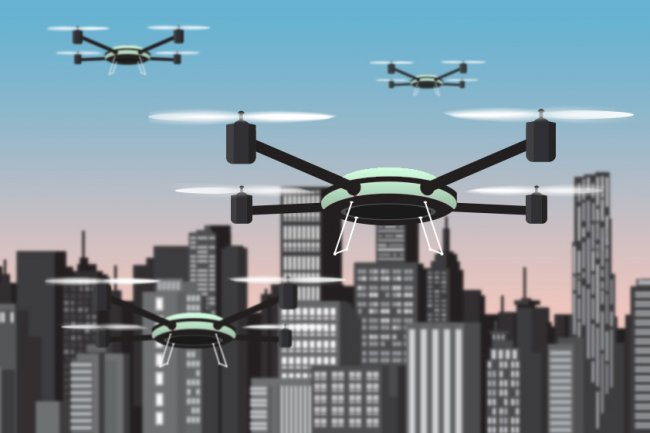
\includegraphics[width=0.8\linewidth]{Images/Evitement d'obstacles}}
		\caption{Évitement d’obstacles}
		\label{fig:my_label}
	\end{minipage}
	\begin{minipage}{0.49\textwidth}
		\fbox{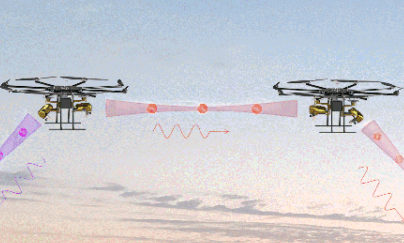
\includegraphics[width=0.8\linewidth]{Images/Quadrirotor mener par un autre}}
		\caption{Suivi de cible}
		\label{fig:my_label}
	\end{minipage}
\end{figure}
\begin{figure}[h]
	\begin{minipage}{0.49\textwidth}
\fbox{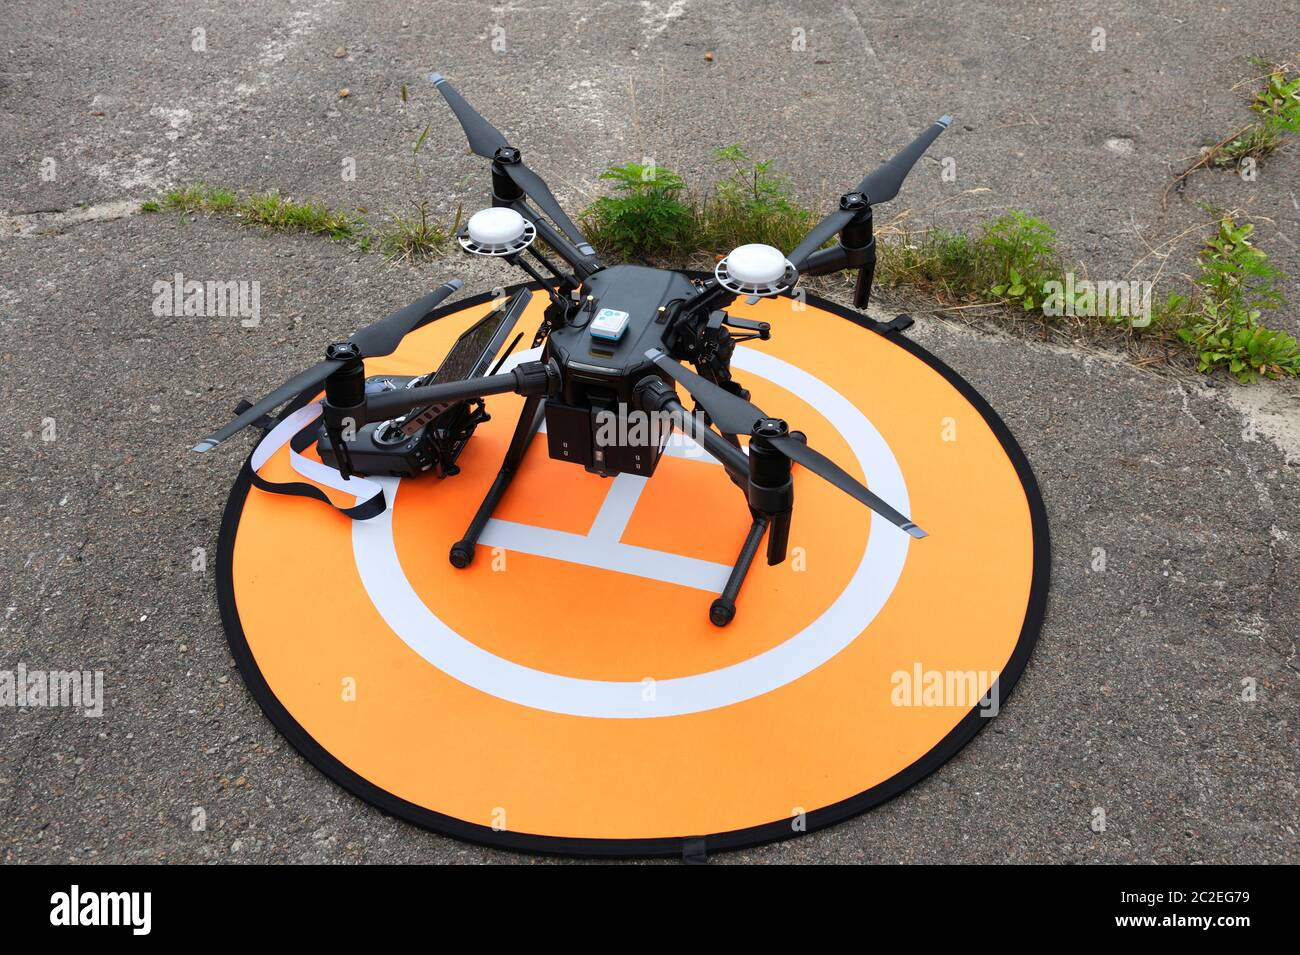
\includegraphics[width=0.8\linewidth]{Images/Atterissage de quadrirotor}}
		\caption{Atterrissage }
		\label{fig:my_label}
	\end{minipage}
	\begin{minipage}{0.49\textwidth}
		\fbox{\includegraphics[width=0.8\linewidth]{Images/Détection d'objet}}
		\caption{Détection d’objets }
		\label{fig:my_label}
	\end{minipage}
\end{figure}
\section{Détection des oranges et comptage}
Notre approche consiste en plusieurs étapes. La première est de détecter les oranges sur des images acquises dans les vergers, par une des méthodes de détection d’objets. Ensuite nous améliorons ces résultats en caractérisant les pixels acquis sur les oranges, puis en estimant une position  dans l’image plus précise pour oranges détectée, ainsi que leur taille moyenne.

\section{Réseau de neurones}

Afin de détecter et catégoriser les objets souhaités, le réseau de neurones à convolutions doit passer par une phase d’apprentissage avant d’être utilisé comme détecteur. Le but de cette dernière est de lui apprendre à reconnaitre une ou plusieurs classes d’objets. Pour cela, nous lui fournissons un ensemble d’images contenant les objets en question que nous aurons encadrés et classifiés au préalable. Ces encadrements sont effectués par nos soins et sont appelés "La vérité sur le terrain" ("Ground Truth" en anglais) qui est le terme technique utilisé dans le domaine de l’IA. Ces "Ground Truth" sont généralement représentés par des rectangles mais peuvent aussi bien être des cercles ou encore des polygones. Et pour chaque "Ground Truth" défini, nous lui associons la classe de l’objet.

\section{Détection d'objet par encadrement}
La plupart des programmes d’IA que nous retrouvons pour la détection et la classification de tous types d’objets, possèdent une architecture utilisant les boîtes englobantes [15]. Le réseau de neurones, après l’analyse de l’image qui est la donnée d’entrée, va nous renvoyer en sortie une image avec des boîtes englobantes encadrant les objets prédits et leurs classes respectives. Ainsi nous avons accès d’une part, à la position de l’objet dans l’image et d’autre part, à sa classe.




\section{Détection des fruits}
La détection et la classification des fruits restent difficiles en raison de la forme, de la couleur et de la texture des différentes espèces de fruits. En étudiant l'impact de la vision par notre système sur la détection et la classification des fruits, nous avons souligné que jusqu'en 2018, de nombreuses méthodes d'apprentissage automatique conventionnelles étaient utilisées tandis que quelques méthodes exploitaient l'application de méthodes d'apprentissage en profondeur pour la détection et la classification des fruits. Cela nous a incités à poursuivre une étude approfondie sur l'enquête et la mise en œuvre de modèles d'apprentissage en profondeur pour la détection et la classification des fruits. Dans cet article, nous avons longuement discuté des ensembles de données utilisés par de nombreux chercheurs, des descripteurs pratiques, de la mise en œuvre du modèle et des défis liés à l'utilisation de l'apprentissage en profondeur pour détecter et catégoriser les fruits. Enfin, nous avons résumé les résultats de différentes méthodes d'apprentissage en profondeur appliquées dans des études antérieures à des fins de détection et de classification des fruits. Cette revue couvre l'étude d'articles récemment publiés qui utilisaient des modèles d'apprentissage en profondeur pour l'identification et la classification des fruits. De plus, nous avons également mis en œuvre à partir de zéro un modèle d'apprentissage en profondeur pour la classification des fruits en utilisant l'ensemble de données populaire "Fruit 360" pour permettre aux chercheurs débutants dans le domaine de l'agriculture de comprendre plus facilement le rôle de l'apprentissage en profondeur dans le domaine de l'agriculture.


\section{Détection des oranges et comptage}

Notre approche consiste en plusieurs étapes. La première est de détecter les oranges sur des images acquises dans les vergers, par une des méthodes de détection d’objets. Ensuite nous améliorons ces résultats en caractérisant les pixels acquis sur les oranges, puis en estimant une position  dans l’image plus précise pour oranges détectée, ainsi que leur taille moyenne.

\section{Détection en temps réel}


\section{Yolo}
Dans un premier temps, étant donné que le modèle de détection doit être à la fois précis et rapide dans son exécution, les outils de détection en temps réel constitue la première approche de ce projet. Selon l’état de l’art, le choix de l’outil YOLO était le plus adéquat. En effet, comme expliqué et montré sur la figure 2.3, l’architecture de YOLO lui permet d’effectuer les tâches de détection et de classification en parallèle, augmentant ainsi sa vitesse d’exécution.

 YOLO découpe l’image en une grille de taille S × S. Puis de façon simultanée, il réalise d’une part la prédiction des objets dans l’image et d’autre part, détermine la classe de l’objet, comme montré sur la figure 2.3.



\section{Conclusion}
Ce chapitre présente d’une manière succincte les définitions et les descriptions des drones. À cet effet, un historique et quelques exemples de ce type d’objets volants ont été présentés  . Dans le chapitre suivant, nous présenterons la modélisation et conception du drone








